\documentclass[]{standalone}
\usepackage{amsmath}
\usepackage{amssymb}
% No page numbers and no paragraph indentation                                  
\pagestyle{empty}                                                               
\setlength{\parindent}{0bp}%
\usepackage{graphicx}
\usepackage{tikz}
\usetikzlibrary{calc,fadings,decorations.pathreplacing,shapes,shapes.multipart,arrows,shapes.misc,intersections,positioning}

\begin{document}

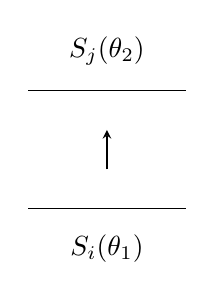
\begin{tikzpicture}[scale = 1]
\draw (0,0)--(2,0);
\draw (0,1.5)--++(2,0);
\node () at (1,-0.5) {$S_i( \theta_1)$};
\node () at (1,2) {$S_j( \theta_2 )$};
\draw[-stealth] (1,0.5)--++(0,0.5);
\end{tikzpicture}

\end{document}

%%% Local Variables: 
%%% TeX-PDF-mode: t
%%% End: 